% In the field of speech processing, speech transcriptions are essential for the performance of speech modeling. 
Speech processing tasks such as automatic speech recognition 
% or speaker identification
have traditionally relied on supervised learning algorithms that require transcribed training data.
However, because transcriptions are expensive and time-consuming to collect, self-supervised speech models have recently become extremely popular. 
Speech models based on self-supervised learning (SSL) can be pre-trained with large amounts of unlabeled data, e.g. using a masked language modeling objective, and subsequently fine-tuned on a relatively small amount of labeled data for a target downstream task. %which relieves the requirements for paired data.
Recent literature has proposed various SSL algorithms~\cite{hsu2021hubert,Chen2021WavLMLS,Conneau2020xlsr,schneider2019wav2vec} and many applications have been built on top of these SSL speech models~\cite{mohamed2022self}, including Automatic Speech Recognition~\cite{baevski2021wav2vec-u,liu2022wav2vec-u2}, Visually Grounded Speech~\cite{peng2022fastvgs,peng2022vghubert,shihSpeechCLIP,layne_mspchclip}, Speech Segmentation~\cite{peng2022vghubert,Strgar_2022}
Emotion recognition~\cite{Morais_emotion_ssl}, speaker verification~\cite{Peng_SSL_sv_2023} and so on.
Furthermore, there are benchmarks proposed to evaluate speech SSL models on various downstream tasks~\cite{yang21c_superb,tsai2022superbsg,shon-etal-2023-slue,shi23g_mlsuperb}.
% \ian{perhaps I should cite more paper using speech SSL models?} \david{It never hurts, although verify that the citations specify the conference/journal version of the paper and not the arxiv version, unless the arxiv version is the only thing that exists at this time. I'd suggest citing one or two for speaker ID/verification and emotion recognition. After that, you can mention benchmarks like SUPERB and SLUE which try to evaluate SSL speech models across a range of different tasks}

\begin{figure}[t]
    \centering
    % 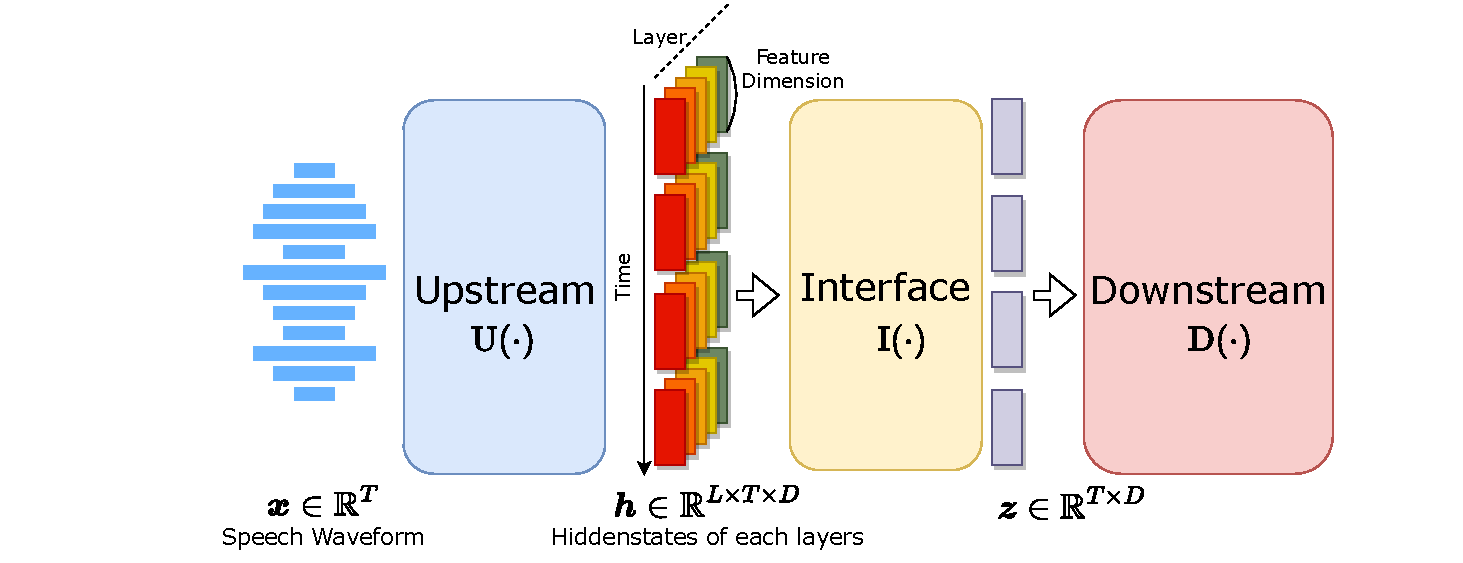
\includegraphics[width=\linewidth,trim={3.7cm 0.25cm 2.1cm 0},clip]{figs/SSL_Interface-Oveview.pdf}
    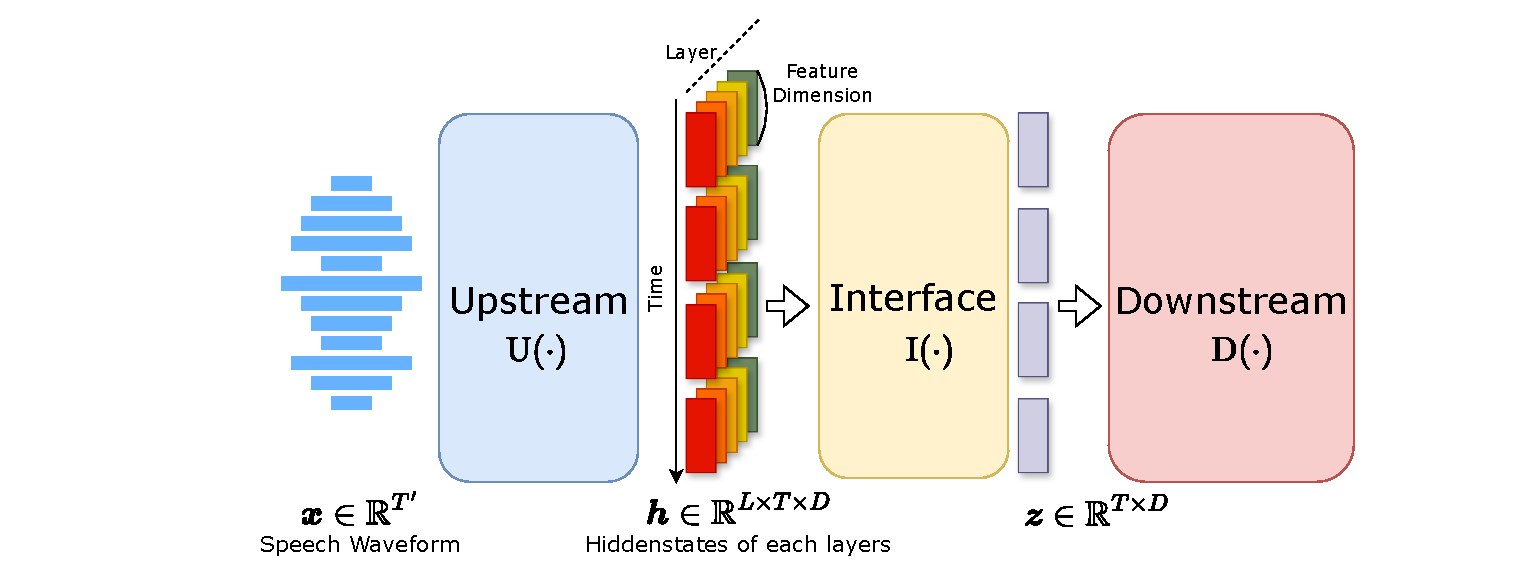
\includegraphics[width=\linewidth,trim={3.7cm 0.25cm 2.1cm 0},clip]{figs/SSL_Interface-Oveview_cameraReady.pdf}
    \caption{The general framework for utilizing self-supervised speech models only considers the upstream and downstream model components. We argue that the interface connecting them should be considered in its own right as a separate component.($L$~:~number of upstream model layers,~$T$~:~upstream model output sequence length,~$D$~:~upstream model feature dimension)}
    \label{fig:framework}
\end{figure}

While significant progress has been made in developing algorithms and applications of speech SSL models, it is still unclear what the best method is for utilizing these models on downstream tasks.
Existing methods for utilizing speech SSL models fall roughly into 3 categories:
1) Cascade the upstream model with a task-specific downstream prediction head and fine-tune the entire model.
2) Freeze the upstream model and take the output of a specific layer as the input features for a task-specific downstream module, then train the downstream module.
3) Compute a learnable weighted sum of all layers belonging to the upstream model and use the result as the input features for a task-specific downstream module. Typically, only the summation weights and the downstream module are trained during fine-tuning.
% Among the three methods, Fine-tuning the upstream and downstream models together often leads to better performance, but the drawbacks are that it is far more computationally expensive and can be unstable when the amount of fine-tuning data is too small.
Among the three methods, Fine-tuning the upstream and downstream models together often leads to better performance, but it is far more computationally expensive and can be unstable when a small amount of fine-tuning data is available.
In contrast, using features from a single layer of the frozen upstream model is the most computationally inexpensive, however, it neglects the non-uniform distribution of different information types encoded across different layers of the upstream model~\cite{Ankita2022CCA}.
The weighted sum can thus be viewed as an intermediate trade-off between the other two options and is the default configuration used in the SUPERB~\cite{yang21c_superb} benchmark.

However, in this paper, we argue that the weighted sum is still a suboptimal way of combining information across layers of speech SSL models.
Our intuition is that because the information encoded in each dimension might differ across each layer of the upstream model, naively summing over the layers dimension-by-dimension may lead to an information loss in proportion to the degree of statistical independence between the same dimension across multiple layers.
%Intuitively, according to the Central Limit Theorem, the sum of random variables will end up approximating a normal distribution as the number of variables gets larger, leading to the loss of information.



Built upon this motivation, we hypothesize that there exists a better way of aggregating the information across different layers and introducing an \textbf{Interface} module in the SSL framework.
The overall framework for utilizing speech SSL models then becomes a set of three components: the
\textbf{Upstream} model, the \textbf{Downstream} prediction head, and the \textbf{Interface} that bridges between them by aggregating information across all upstream model layers.
% Under this definition, we can see that the widely-used weighted sum method is a specific type of interface, and in this paper we further propose several alternative interface designs.
Under this definition, the widely-used weighted sum method is a specific type of interface, and in this paper, we further propose several alternative interface designs.
% , including multiple groups of weighted sum, using PCA to do dimension reduction on each layer before concatenating, performing convolution calculation across layer dimension and so on.
We evaluate the performance of each proposed interface across 5 upstream speech SSL models and several downstream tasks in the ML-SUPERB~\cite{shi23g_mlsuperb} and SUPERB~\cite{yang21c_superb} benchmarks.
Among all our proposed interfaces, we show that Hierarchical Convolution across layers tends to achieve the best overall performance.
We also conduct additional experiments showing that performance differences among various interface designs are due to their architectures themselves, and are not merely due to the difference in the number of trainable parameters.
Additionally, we show that the Hierarchical Convolution interface still outperforms the weighted sum interface when the upstream model is fine-tuned with the downstream model.
The code is publicly available.
\footnote{\url{https://github.com/atosystem/SSL_Interface}}
Our contributions in this paper can be summarized as follows:
\begin{enumerate}
    \item We propose an updated framework for self-supervised speech models that formally recognizes the interface module
    \item We introduce several designs for the interface and show that the Hierarchical Convolution tends to perform the best across many speech processing tasks
    \item We show that even when the full model is end-to-end fine-tuned, different interfaces still show performance differences.
\end{enumerate}